\documentclass{beamer}
\usepackage{ctex} %采用中文
\usepackage{hyperref} %超链接
\usepackage[T1]{fontenc}

\usepackage{latexsym,xcolor,multicol,booktabs}
\usepackage{graphicx,pstricks,listings,stackengine}
\usepackage{linguex,cgloss4e,tikz,qtree,tikz-qtree}
\usetikzlibrary{graphs}

\usepackage{calligra} %英文字体
%中西文混排字库New Century Schoolbook
\usepackage[p,scaled=0.95]{scholax} % 0.95 适合与汉字匹配, osf 风格有效
\usepackage[scaled=.99]{helvet} % text = Helvetica = sans serif
\usepackage{amsmath,amsthm} % 数学符号,要在newtxmath之前
\usepackage[scaled=.95,ncf,varbb]{newtxmath} % need to scale up math package: vvarbb

% 设置用acrobat打开就会全屏显示
\hypersetup{pdfpagemode=FullScreen}

% 设置logo
\pgfdeclareimage[height=0.8cm]{university-logo}{pic/BNU_com} %需提前将logo文件放到`.tex`文件中。
\logo{\pgfuseimage{university-logo}}

\author[Yuxuan Liu]{某某某}
\title{BNU Beamer Theme}
\subtitle{北京师范大学毕业论文答辩}
\institute[北京师范大学 文学院]{文学院\\语言学及应用语言学研究所}
\date{2023年4月29日}
\usepackage{BNU_beamer_theme}

% defs
\def\cmd#1{\texttt{\color{red}\footnotesize $\backslash$#1}}
\def\env#1{\texttt{\color{blue}\footnotesize #1}}
\definecolor{deepblue}{rgb}{0,0,0.5}
\definecolor{deepred}{rgb}{0.6,0,0}
\definecolor{deepgreen}{rgb}{0,0.5,0}
\definecolor{halfgray}{gray}{0.55}

\lstset{
    basicstyle=\ttfamily\small,
    keywordstyle=\bfseries\color{deepblue},
    emphstyle=\ttfamily\color{deepred},    % Custom highlighting style
    stringstyle=\color{deepgreen},
    numbers=left,
    numberstyle=\small\color{halfgray},
    rulesepcolor=\color{red!20!green!20!blue!20},
    frame=shadowbox,
}

% defs
\def\cmd#1{\texttt{\color{red}\footnotesize $\backslash$#1}}
\def\env#1{\texttt{\color{blue}\footnotesize #1}}
\definecolor{deepblue}{rgb}{0,0,0.5}
\definecolor{deepred}{rgb}{0.6,0,0}
\definecolor{deepgreen}{rgb}{0,0.5,0}
\definecolor{halfgray}{gray}{0.55}

\begin{document}

\AtBeginSection[]
{
 \begin{frame}
 \frametitle{章节目录}
 \begin{multicols}{2}
  \tableofcontents[currentsection]
 \end{multicols}
 \end{frame}
}

\AtBeginSubsection[]
{
 \begin{frame}
 \frametitle{章节目录}
 \begin{multicols}{2}
  \tableofcontents[currentsection]
 \end{multicols}
 \end{frame}
}

\begin{frame}
    %\maketitle
    \titlepage
    %\begin{figure}[htpb] %居中校徽,如果去除统一虚化背景建议在这里加上
        %\begin{center}
        %    
\includegraphics[width=0.2\linewidth]{pic/Beijing_Normal_University_Logo.eps}
        %\end{center}
    %\end{figure}
\end{frame}

\begin{frame}
    \frametitle{总目录}
    \begin{multicols}{2}
     \tableofcontents[hideallsubsections]
    \end{multicols}
\end{frame}

\section{选题缘起}
\subsection{Beamer的优势}
\begin{frame}{为什么是Beamer}
    \begin{itemize}[<+-| alert@+>] % alert 用于逐帧动画,也可以手动在里面插 \pause ,不需要可以删除
        \item 利用\LaTeX{},快速将论文浓缩成演示文档
        \item 中文支持请选择 Xe\LaTeX{} 编译选项 
        \item Overleaf项目地址暂时木有
        \item GitHub项目地址暂时木有
    \end{itemize}
\end{frame}

\begin{frame}{Why Beamer}
    \begin{itemize}
        \item \LaTeX 广泛用于学术界,期刊会议论文模板
    \end{itemize}
    \begin{table}[h]
        \centering
        \begin{tabular}{c|c}
            Microsoft\textsuperscript{\textregistered}  Word & \LaTeX \\
            \hline
            文字处理工具 & 专业排版软件 \\
            容易上手,简单直观 & 容易上手 \\
            所见即所得 & 所见即所想,所想即所得 \\
            高级功能不易掌握 & 进阶难,但一般用不到 \\
            处理长文档需要丰富经验 & 和短文档处理基本无异 \\
            花费大量时间调格式 & 无需担心格式,专心作者内容 \\
            公式排版差强人意 & 尤其擅长公式排版 \\
            二进制格式,兼容性差 & 文本文件,易读、稳定 \\
            付费商业许可 & 自由免费使用 \\
        \end{tabular}
    \end{table}
\end{frame}

\section{研究现状}

\subsection{Beamer主题分类}
\begin{frame}
    \begin{itemize}
        \item 有一些 \LaTeX{} 自带的
        \item 有一些其他高校的主题
        \item 本模板基于清华大学模板 \href{https://github.com/tuna/THU-Beamer-Theme}{\color{bnu} $THUlink$} \cite{thu} 进行修改
        \item 校徽布局参考大连理工大学模板 \href{https://github.com/fuujiro/DLUT-Beamer-Slide-V1/tree/master}{\color{bnu} $DLUTlink$} \cite{dlut}
        \item 主体色调参考2007年《北京师范大学视觉形象识别系统手册》“师大蓝” 
        \newline 师大蓝(深蓝) C100 M70 Y0 K0 用于标志和中英文名称
        \newline 师大蓝(浅蓝) C100 M30 Y0 K0 用于背景色、配色
    \end{itemize}
\end{frame}


\section{研究内容}

\begin{frame}{本主题对THU Beamer Theme的改动在于}
    \begin{itemize}
        \item 顶栏导航变成多行而非一行
        \item 主要内容中文采用宋体,英文采用罗马体
        \item 置换了标志,主体色调采用师大蓝
        \item 目录由单栏改为双栏
        \item 外部主题以miniframes替代smoothbars,取消了颜色过渡
        \item 打开命令行Win + R,输入"texdoc beamer",在官方文档中探索更多功能
    \end{itemize}
\end{frame}

\subsection{排版举例}

\begin{frame}{公式与编号}
    带编号的公式:
    \begin{equation}
        f(x) = \frac{\mathrm e^{2x}}{\sin x}
        \end{equation}
    不带编号的公式:
    \begin{equation*}
        J(\theta) = \mathbb{E}_{\pi_\theta}[G_t] = \sum_{s\in\mathcal{S}} d^\pi (s)V^\pi(s)=\sum_{s\in\mathcal{S}} d^\pi(s)\sum_{a\in\mathcal{A}}\pi_\theta(a|s)Q^\pi(s,a)
    \end{equation*}
    以及一个行内公式$a^2 + b^2 = c^2$.
\end{frame}

\begin{frame}{公式与编号}
    多行多列公式 %如果公式中有文字出现,请用 $\backslash$mathrm\{\} 或者 $\backslash$text\{\} 包含,不然就会变成 $clip$,在公式里看起来比 $\mathrm{clip}$ 丑非常多
    % 使用 & 分隔
    \begin{align}
            Q_\mathrm{target}&=r+\gamma Q^\pi(s^\prime, \pi_\theta(s^\prime)+\epsilon)\\
            \epsilon&\sim\mathrm{clip}(\mathcal{N}(0, \sigma), -c, c)\nonumber
    \end{align}
\end{frame}

\begin{frame}{图形与分栏}
    % From thuthesis user guide.
    \begin{minipage}[c]{0.3\linewidth}
        \psset{unit=0.8cm}
        \begin{pspicture}(-1.75,-3)(3.25,4)
            \psline[linewidth=0.25pt](0,0)(0,4)
            \rput[tl]{0}(0.2,2){$\vec e_z$}
            \rput[tr]{0}(-0.9,1.4){$\vec e$}
            \rput[tl]{0}(2.8,-1.1){$\vec C_{ptm{ext}}$}
            \rput[br]{0}(-0.3,2.1){$\theta$}
            \rput{25}(0,0){%
            \psframe[fillstyle=solid,fillcolor=lightgray,linewidth=.8pt](-0.1,-3.2)(0.1,0)}
            \rput{25}(0,0){%
            \psellipse[fillstyle=solid,fillcolor=yellow,linewidth=3pt](0,0)(1.5,0.5)}
            \rput{25}(0,0){%
            \psframe[fillstyle=solid,fillcolor=lightgray,linewidth=.8pt](-0.1,0)(0.1,3.2)}
            \rput{25}(0,0){\psline[linecolor=red,linewidth=1.5pt]{->}(0,0)(0.,2)}
%           \psRotation{0}(0,3.5){$\dot\phi$}
%           \psRotation{25}(-1.2,2.6){$\dot\psi$}
            \psline[linecolor=red,linewidth=1.25pt]{->}(0,0)(0,2)
            \psline[linecolor=red,linewidth=1.25pt]{->}(0,0)(3,-1)
            \psline[linecolor=red,linewidth=1.25pt]{->}(0,0)(2.85,-0.95)
            \psarc{->}{2.1}{90}{112.5}
            \rput[bl](.1,.01){C}
        \end{pspicture}
    \end{minipage}\hspace{1cm}
    \begin{minipage}{0.5\linewidth}
        \medskip
        %\hspace{2cm}
        \begin{figure}[h]
            \centering
            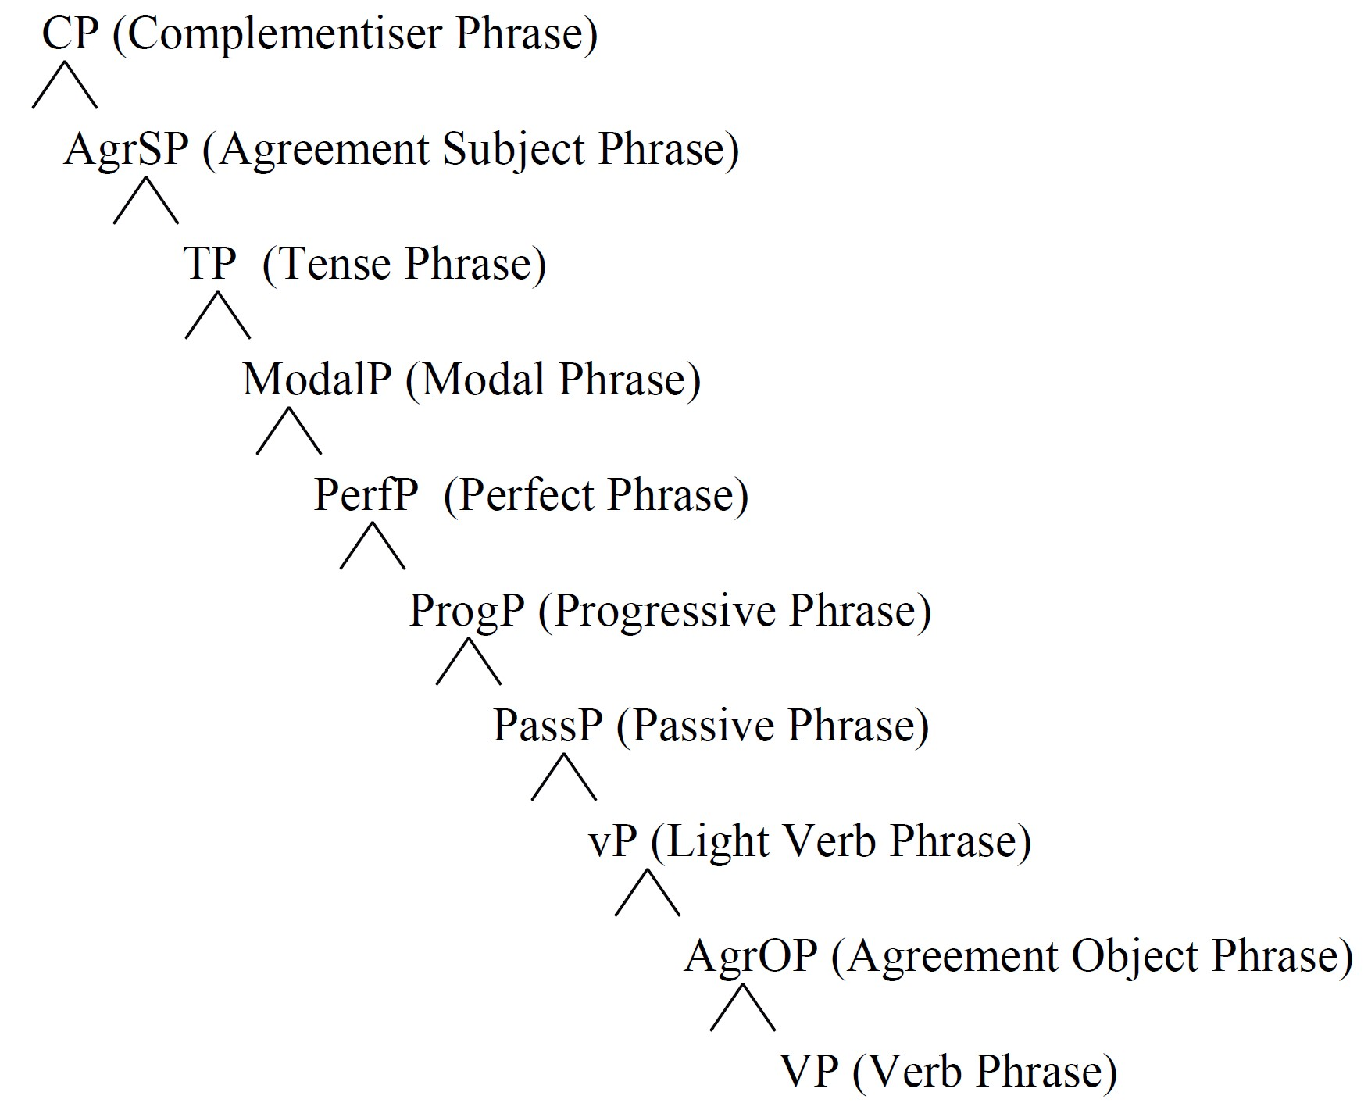
\includegraphics[height=5cm]{pic/fq_syn.pdf}
        \end{figure}
    \end{minipage}
\end{frame}

\begin{frame}[fragile]{\LaTeX{} 常用命令}
    \begin{exampleblock}{命令}
        \centering
        \footnotesize
        \begin{tabular}{llll}
            \cmd{chapter} & \cmd{section} & \cmd{subsection} & \cmd{paragraph} \\
            章 & 节 & 小节 & 带题头段落 \\\hline
            \cmd{centering} & \cmd{emph} & \cmd{verb} & \cmd{url} \\
            居中对齐 & 强调 & 原样输出 & 超链接 \\\hline
            \cmd{footnote} & \cmd{item} & \cmd{caption} & \cmd{includegraphics} \\
            脚注 & 列表条目 & 标题 & 插入图片 \\\hline
            \cmd{label} & \cmd{cite} & \cmd{ref} \\
            标号 & 引用参考文献 & 引用图表公式等\\\hline
        \end{tabular}
    \end{exampleblock}
    \begin{exampleblock}{环境}
        \centering
        \footnotesize
        \begin{tabular}{lll}
            \env{table} & \env{figure} & \env{equation}\\
            表格 & 图片 & 公式 \\\hline
            \env{itemize} & \env{enumerate} & \env{description}\\
            无编号列表 & 编号列表 & 描述 \\\hline
        \end{tabular}
    \end{exampleblock}
\end{frame}

\begin{frame}[fragile]{\LaTeX{} 环境命令举例}
    \begin{minipage}{0.5\linewidth}
\begin{lstlisting}[language=TeX]
\begin{itemize}
  \item A \item B
  \item C
  \begin{itemize}
    \item C-1
  \end{itemize}
\end{itemize}
\end{lstlisting}
    \end{minipage}\hspace{1cm}
    \begin{minipage}{0.3\linewidth}
        \begin{itemize}
            \item A
            \item B
            \item C
            \begin{itemize}
                \item C-1
            \end{itemize}
        \end{itemize}
    \end{minipage}
    \medskip
    \pause
    \begin{minipage}{0.5\linewidth}
\begin{lstlisting}[language=TeX]
\begin{enumerate}
  \item 巨佬 \item 大佬
  \item 萌新
  \begin{itemize}
    \item[n+e] 瑟瑟发抖
  \end{itemize}
\end{enumerate}
\end{lstlisting}
    \end{minipage}\hspace{1cm}
    \begin{minipage}{0.3\linewidth}
        \begin{enumerate}
            \item 巨佬
            \item 大佬
            \item 萌新
            \begin{itemize}
                \item[n+e] 瑟瑟发抖
            \end{itemize}
        \end{enumerate}
    \end{minipage}
\end{frame}

\begin{frame}[fragile]{\LaTeX{} 数学公式}
    \begin{columns}
        \begin{column}{.55\textwidth}
\begin{lstlisting}[language=TeX]
$V = \frac{4}{3}\pi r^3$

\[
  V = \frac{4}{3}\pi r^3
\]

\begin{equation}
  \label{eq:vsphere}
  V = \frac{4}{3}\pi r^3
\end{equation}
\end{lstlisting}
        \end{column}
        \begin{column}{.4\textwidth}
            $V = \frac{4}{3}\pi r^3$
            \[
                V = \frac{4}{3}\pi r^3
            \]
            \begin{equation}
                \label{eq:vsphere}
                V = \frac{4}{3}\pi r^3
            \end{equation}
        \end{column}
    \end{columns}
    \begin{itemize}
        \item 更多内容请看 \href{https://zh.wikipedia.org/wiki/Help:数学公式}{\color{bnu}{这里}}
    \end{itemize}
\end{frame}

\begin{frame}[fragile]
    \frametitle{制表}
    \begin{columns}
        \column{.6\textwidth}
\begin{lstlisting}[language=TeX]
    \begin{table}[htbp]
      \caption{编号与含义}
      \label{tab:number}
      \centering
      \begin{tabular}{cl}
        \toprule
        编号 & 含义 \\
        \midrule
        1 & 4.0 \\
        2 & 3.7 \\
        \bottomrule
      \end{tabular}
    \end{table}
\end{lstlisting}
        \column{.4\textwidth}
        \begin{table}[htpb]
            \centering
            \caption{编号与含义}
            \label{tab:number}
            \begin{tabular}{cl}\toprule
                编号 & 含义 \\\midrule
                1 & 4.0\\
                2 & 3.7\\\bottomrule
            \end{tabular}
        \end{table}
        \normalsize 公式~(\ref{eq:vsphere})的编号与含义请参见表~\ref{tab:number}。
    \end{columns}
\end{frame}

\begin{frame}{作图}
    \begin{itemize}
        \item 矢量图 eps, ps, pdf
        \begin{itemize}
            \item METAPOST, pstricks, pgf $\ldots$
            \item Xfig, Dia, Visio, Inkscape $\ldots$
            \item Matlab / Excel 等保存为 pdf
        \end{itemize}
        \item 标量图 png, jpg, tiff $\ldots$
        \begin{itemize}
            \item 提高清晰度,避免发虚
            \item 应尽量避免使用
        \end{itemize}
    \end{itemize}
    \begin{figure}[htpb]
        \centering
        
\includegraphics[width=0.2\linewidth]{pic/Beijing_Normal_University_Logo.eps}
        \caption{这个校徽就是矢量图}
    \end{figure}
\end{frame}

\begin{frame}{作图}
    \ex. \leavevmode\vadjust{\vspace{-\baselineskip}}\newline
    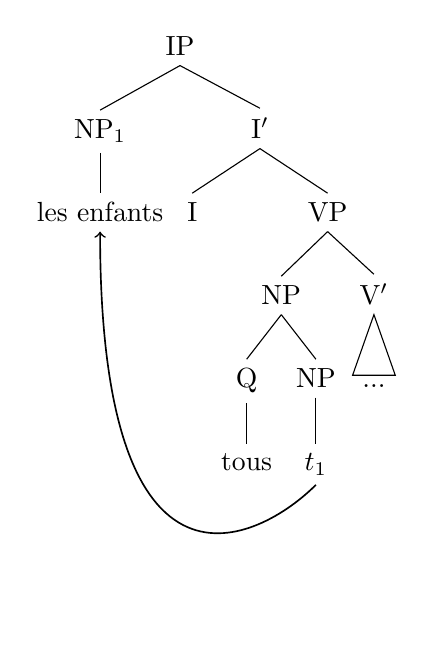
\begin{tikzpicture}
        \Tree [.IP [.NP$_1$ \node(np){les~enfants}; ]
                [.I$'$ [.I ]
                       [.VP [.NP [.Q tous ]
                                 [.NP \node(t){$t_1$}; ] ] 
                            [.V$'$ \edge[roof]; {...} ] ] ] ]
        \draw[semithick,->] (t.south)..controls +(south west:1) and +(south:5)..(np.south);
    \end{tikzpicture}
    \par
    % 关于tikz制图详见\url{https://ftp.yz.yamagata-u.ac.jp/pub/CTAN/graphics/pgf/base/doc/pgfmanual.pdf}
    % 关于语料标注详见\url{https://zhuanlan.zhihu.com/p/399744454}
\end{frame}

\section{研究结论}
\begin{frame}{研究结论}
    \begin{itemize}
        \item 新发现
        \item 新方法
        \item 新材料
        \item ...
    \end{itemize}
\end{frame}

\section{参考文献}

\begin{frame}{References}%[allowframebreaks]
    \bibliography{ref}
    \bibliographystyle{alpha}
    % 如果参考文献太多的话,可以像下面这样调整字体:
    % \tiny\bibliographystyle{alpha}
\end{frame}

\begin{frame}{结语}
    \begin{center}
        {\Huge\calligra Thanks!}
    \end{center}
\end{frame}

\end{document}